%!TEX root = uist14.tex
\section{Iteration 2: IR Intensity refinement}

\bjoern{The results of the first study show that head orientation targeting can outperform linear list selection, but that disambiguation (or refinement step, need to decide on consistent terminology) is costly.

Our approach to avoid paying this penalty is to provide more information to the system which target is more likely than another to be the intended selection. We do so by collecting received IR signal strength at each target node and comparing measurements of all candidate targets.}

\subsection{Interaction Flow}
\bjoern{
Intensity data is used in two ways (see Figure~\ref{fig:selectflow02}): 1) the difference in intensity between the strongest and second target exceeds a threshold, the target with the strongest received signal is automatically selected; 2) if the difference falls below the threshold, the refinement UI from the previous iteration is displayed, but items are ordered in decreasing intensity. This should maximize the chance of being able to confirm the intended target without additional UI navigation actions}.


\begin{figure}[t]
\centering
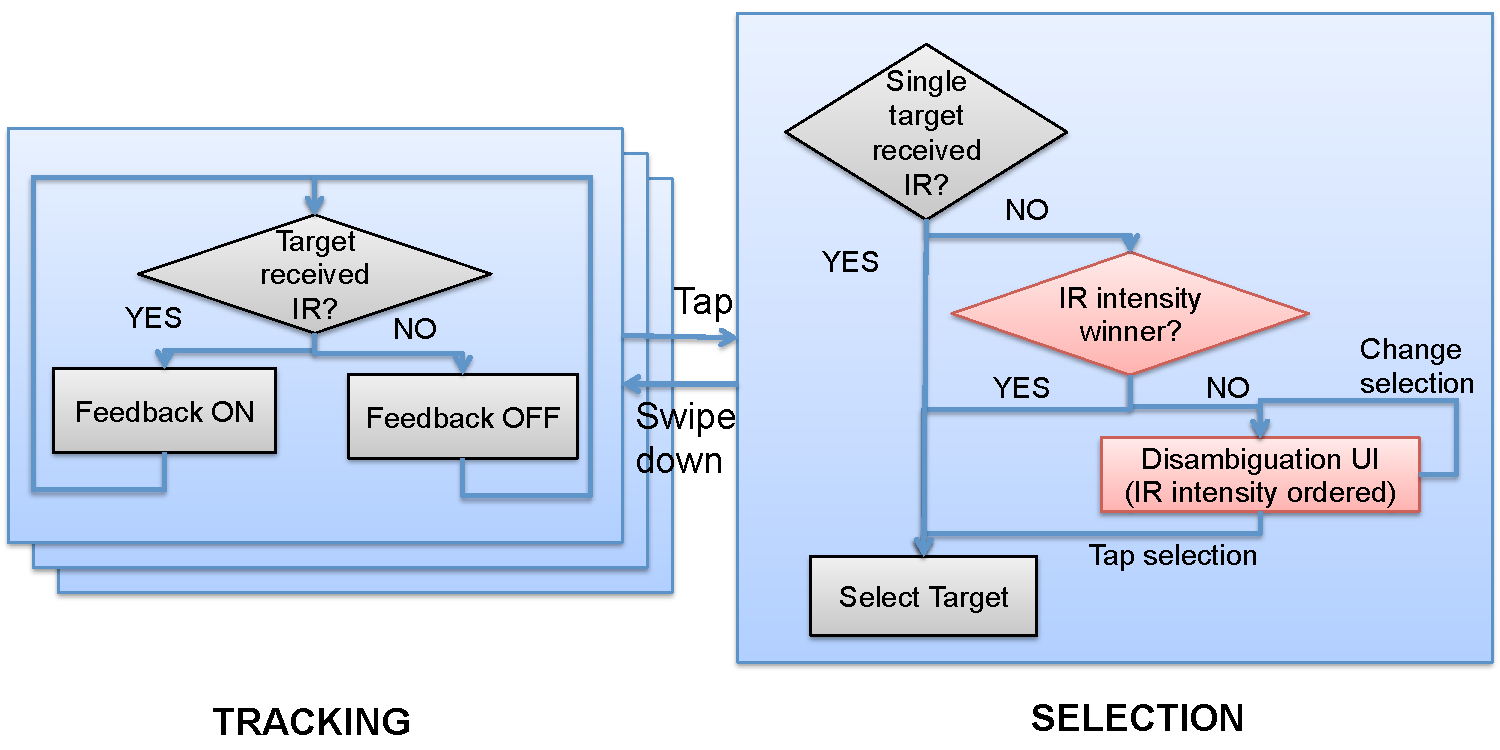
\includegraphics[width=1.0\columnwidth]{figures/selectflow02.pdf}
\caption{Head orientation selection flowchart for our second design with IR intensity measurement.}
\label{fig:selectflow02}
\end{figure}

\subsection{Implementation}
\bjoern{we use sensor X and LED y which give useful readings at up to N feet. Intensity falls of as $1/d^2$ with distance and approximately $xyz$ with angle. We empirically set the threshold for automatic selection without refinement at Z.}\bjoern{maybe show some measurements for intensity based on distance and angle as we had discussed a while ago. not essential. }
